% 1. ročník MAT – příprava 101; inspirace Realisticky.cz 020501–020506, úlohy nově sestavené.
\documentclass[11pt,a4paper]{article}
\input{../../sablony/pripravy/priprava.sty}
\usepackage{tikz}
\usepackage{pgfplots}
\pgfplotsset{compat=1.18}
\usetikzlibrary{arrows.meta}
\nastavPripravu{1. ročník}{Kvadratické funkce}{101}{Graf z obecného předpisu}
\begin{document}
\blok{Sestrojit celý graf z obecného předpisu}
Pro $f(x)=ax^2+bx+c$ můžeme najít vrchol doplněním na čtverec, osu souměrnosti, průsečík s osou $y$ a další kontrolní body. Pokud je rozklad jednoduchý, přidáme i průsečíky s osou $x$. Parabolu kreslíme souměrně, nikoliv jako lomenou čáru.
\blok{Přehled algoritmu}
\begin{enumerate}[label=\arabic*.]
\item Uprav $ax^2+bx+c$ na vrcholový tvar $a(x-m)^2+n$.
\item Vyznač vrchol $V[m;n]$ a osu souměrnosti $x=m$; určete orientaci a obor hodnot.
\item Vyznač průsečík s osou $y$: $[0;c]$; jeho obraz souměrný kolem $x=m$ leží také na grafu.
\item Podle potřeby dopočítej další body a jednodušší nulové body. Spoj body plynulou parabolou.
\end{enumerate}
\blok{Společně řešené příklady}

\begin{prikladReseniBox}
Sestrojte graf $f(x)=x^2-4x+3$. Určete vrchol, osu, $H(f)$ a průsečíky s osami.
\tcblower
\[
\begin{aligned}
f(x)&=x^2-4x+3=(x-2)^2-1 \\
V&=[2;-1],\quad\text{osa: }x=2 \\
H(f)&=\langle-1;+\infty) \\
P_y&=[0;3],\quad \text{souměrný bod }[4;3] \\
f(x)=0&\iff(x-1)(x-3)=0 \\
P_{x,1}&=[1;0],\quad P_{x,2}=[3;0]
\end{aligned}
\]

\end{prikladReseniBox}
\begin{center}
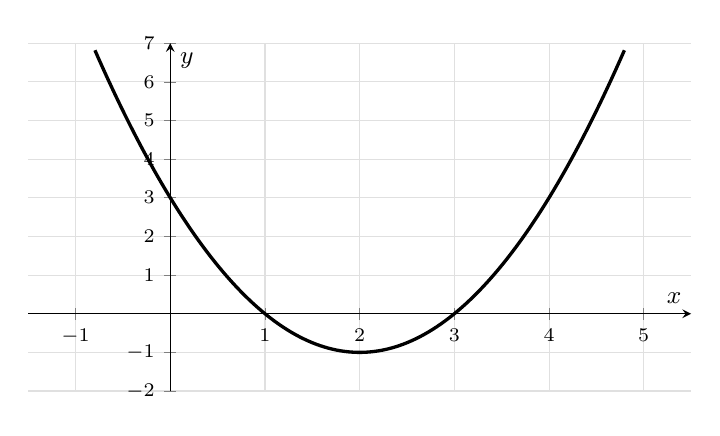
\begin{tikzpicture}
\begin{axis}[
width=10cm,height=6.0cm,axis lines=middle,
xmin=-1.5,xmax=5.5,ymin=-2,ymax=7,
xtick={-1,0,...,5},ytick={-2,-1,...,7},grid=both,
minor tick num=0,grid style={black!12},
tick label style={font=\scriptsize},xlabel={$x$},ylabel={$y$},
label style={font=\small},restrict y to domain=-2:7,
clip=true,legend style={font=\scriptsize,draw=none,fill=none,at={(0.98,0.98)},anchor=north east},
]
\addplot[very thick,solid,domain=-1.5:5.5,samples=160] {x^2-4*x+3};
\end{axis}
\end{tikzpicture}
\end{center}
\begin{prikladReseniBox}
Sestrojte graf $g(x)=-x^2-2x+3$ a vysvětlete, proč se parabola obrací dolů.
\tcblower
\[
\begin{aligned}
g(x)&=-(x^2+2x)+3 \\
&=-(x+1)^2+4 \\
V&=[-1;4],\quad H(g)=(-\infty;4\rangle \\
P_y&=[0;3],\quad\text{souměrný bod }[-2;3] \\
g(x)=0&\iff -(x+3)(x-1)=0 \\
P_{x,1}&=[-3;0],\quad P_{x,2}=[1;0]
\end{aligned}
\]

\end{prikladReseniBox}
\blok{Samostatná práce: celý postup}

\begin{zadaniReseniBox}
a) U $h(x)=2x^2-8x+6$ určete vrchol, osu, obor hodnot, průsečíky s osami a proveďte náčrt.\par
b) U $k(x)=x^2+4x+5$ určete totéž a vysvětlete, proč nemá nulový bod.
\tcblower
\[
\begin{aligned}
h(x)&=2(x-2)^2-2,\quad V_h=[2;-2] \\
H(h)&=\langle-2;+\infty),\ P_y[0;6] \\
h(x)=0&\iff2(x-1)(x-3)=0\Rightarrow x\in\{1;3\} \\
k(x)&=(x+2)^2+1,\quad V_k=[-2;1] \\
H(k)&=\langle1;+\infty),\quad P_y[0;5] \\
k(x)&>0\ \Rightarrow\ \text{nemá nulový bod.}
\end{aligned}
\]

\end{zadaniReseniBox}
\blok{Volitelná rezerva}
Vyznačte pro $y=x^2-4x+3$ všechny argumenty, pro které je funkční hodnota záporná, \emph{jen z grafu}. Výsledek $1<x<3$ je předzvěstí budoucích kvadratických nerovnic; zatím jej z grafu pouze odečtěte.
\blok{Domácí úkol}
\begin{zadaniReseniBox}[title={Domácí příprava}]
\begin{enumerate}[label=\alph*),itemsep=3pt]
\item U funkce $f(x)=x^2-2x-3$ vypočtěte vrchol a průsečík s osou $y$.
\item Naskicujte $y=-x^2+4x$; určete vrchol, osu a nulové body.
\item U $y=2x^2+4x+3$ stanovte vrchol a obor hodnot. Má nulový bod?
\item Sestrojte $y=-x^2-2x+8$ přes vrchol a průsečíky s osami.
\item Pro $y=\tfrac12x^2-2x+1$ určete vrchol, osu a $H(f)$.
\item U $y=(x+3)^2-4$ napište obecný tvar a určete průsečíky s osami.
\item \textbf{Výzva:} Pro $f(x)=x^2-4x+3$ a $D(f)=\langle0;1\rangle$ určete skutečný obor hodnot.
\end{enumerate}
\tcblower
\begin{enumerate}[label=\alph*),itemsep=4pt]
\item
\[
\begin{aligned}
f(x)&=(x-1)^2-4 \\
V&=[1;-4],\quad P_y[0;-3]
\end{aligned}
\]

\item
\[
\begin{aligned}
-x^2+4x&=-(x-2)^2+4 \\
V&=[2;4],\quad\text{osa: }x=2 \\
K&=\{0;4\}
\end{aligned}
\]

\item
\[
\begin{aligned}
2x^2+4x+3&=2(x+1)^2+1 \\
V&=[-1;1],\quad H=\langle1;+\infty) \\
K&=\varnothing
\end{aligned}
\]

\item
\[
\begin{aligned}
-x^2-2x+8&=-(x+1)^2+9 \\
V&=[-1;9],\quad P_y[0;8] \\
0&=-(x+4)(x-2)\Rightarrow x\in\{-4;2\}
\end{aligned}
\]

\item
\[
\begin{aligned}
\tfrac12x^2-2x+1&=\tfrac12(x-2)^2-1 \\
V&=[2;-1],\quad\text{osa: }x=2 \\
H(f)&=\langle-1;+\infty)
\end{aligned}
\]

\item
\[
\begin{aligned}
(x+3)^2-4&=x^2+6x+5 \\
P_y&=[0;5] \\
x+3&=\pm2\Rightarrow x\in\{-5;-1\}
\end{aligned}
\]

\item
\[
\begin{aligned}
f(0)&=3,\quad f(1)=0 \\
\text{Na }\langle0;1\rangle&\text{ je }f\text{ klesající} \\
H(f)&=\langle0;3\rangle
\end{aligned}
\]

\end{enumerate}
\end{zadaniReseniBox}
\poznamka{Čas: algoritmus 5 min, první graf 14 min, druhý příklad 10 min, samostatná práce 12 min, kontrola 4 min. Obtížnější nulové body nenuť počítat vzorcem; vždy stačí srozumitelná konstrukce z vrcholového tvaru a dalších bodů.}
\end{document}
